
\begin{enumerate}
\item Let $\vec{A}=\myvec{7\\-2}, \vec{B}=\myvec{5 \\ 1}, \vec{C}=\myvec{3 \\ k}$\\
The direction vectors of AB and AC are
\begin{align}
\label{aug/2/10/eq:1}
\vec{B} - \vec{A} ={}& \myvec{-2 \\ 3}\\
\label{aug/2/10/eq:2}
\vec{C} - \vec{A} ={}& \myvec{-4 \\ k+2}
\end{align}

\begin{align}
\label{aug/2/10/eq:3}
\vec{M} =\myvec{\vec{B}-\vec{A} & \vec{C}-\vec{A}}^\top
\end{align}
Substituting \eqref{aug/2/10/eq:1} and \eqref{aug/2/10/eq:2} in \eqref{aug/2/10/eq:3}, we get
\begin{align}
\label{aug/2/10/eq:4}
\vec{M}={}&\myvec{-2 & 3 \\ -4 & k+2}
\end{align}
We know that if $rank\brak{\vec{M}}=1$, the points are collinear.
Finding the rank of the matrix in the problem,
\begin{align}
\label{aug/2/10/eq:5}
\vec{M} = \myvec{-2 & 3 \\ -4 & k+2} \overset{R_{2}\rightarrow R_{2}-2R_{1}}{\longleftrightarrow} \myvec{-2 & 3 \\ 0 & k-4}
\end{align}
Since $rank\brak{\vec{M}}=1$, the number of non zero rows left after doing row operations should be equal to 1.
Since row 1 in \eqref{aug/2/10/eq:5} is non zero, elements row 2 should be equal to 0.
\begin{align}
\therefore k=4
\end{align}
\begin{figure}[!h]
\centering
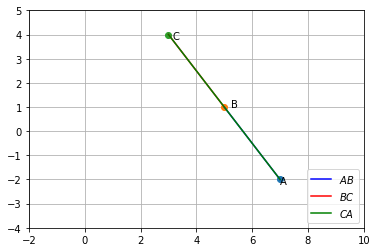
\includegraphics[width=\columnwidth]{solutions/aug/2/10/Figures/q1a.png}
\caption{Plot of the line}
\end{figure}



\item Let $\vec{A}=\myvec{8\\1}, \vec{B}=\myvec{k \\ -4}, \vec{C}=\myvec{2 \\ -5}$\\
The direction vectors of AB and AC are
\begin{align}
\label{aug/2/10/eq:7}
\vec{B} - \vec{A} ={}& \myvec{k-8\\-5}\\
\label{aug/2/10/eq:8}
\vec{C} - \vec{A} ={}& \myvec{-6 \\ -6}
\end{align}
\begin{align}
\label{aug/2/10/eq:9}
\vec{M} =\myvec{\vec{B}-\vec{A} & \vec{C}-\vec{A}}^\top
\end{align}
Substituting \eqref{aug/2/10/eq:7} and \eqref{aug/2/10/eq:8} in \eqref{aug/2/10/eq:9}, we get
\begin{align}
\label{aug/2/10/eq:10}
\vec{M}={}&\myvec{k-8 & -5 \\ -6 & -6}
\end{align}
We know that if $rank\brak{\vec{M}}=1$, the points are collinear.
Finding the rank of the matrix in the problem,
\begin{align}
\label{aug/2/10/eq:11}
\vec{M} = \myvec{k-8 & -6 \\ -5 & -6} \overset{R_{2}\rightarrow 5R_{2}-6R_{1}}{\longleftrightarrow} \myvec{k-8 & -5 \\ 18-6k & 0}
\end{align}
Since $rank\brak{\vec{M}}=1$, the number of non zero rows left after doing row operations should be equal to 1.
Since row 1 in \eqref{aug/2/10/eq:11} is non zero for any value of k , elements row 2 should be equal to 0.
\begin{align}
\therefore k=3
\end{align}

\begin{figure}[!h]
\centering
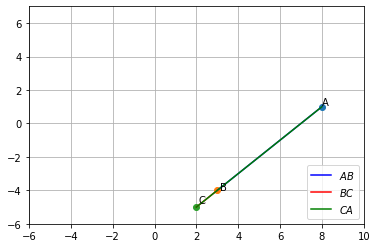
\includegraphics[width=\columnwidth]{solutions/aug/2/10/Figures/q1b.png}
\caption{Plot of the line}
\end{figure}

\end{enumerate}



